% Options for packages loaded elsewhere
\PassOptionsToPackage{unicode}{hyperref}
\PassOptionsToPackage{hyphens}{url}
\PassOptionsToPackage{dvipsnames,svgnames,x11names}{xcolor}
%
\documentclass[
  letterpaper,
  DIV=11,
  numbers=noendperiod]{scrartcl}

\usepackage{amsmath,amssymb}
\usepackage{lmodern}
\usepackage{iftex}
\ifPDFTeX
  \usepackage[T1]{fontenc}
  \usepackage[utf8]{inputenc}
  \usepackage{textcomp} % provide euro and other symbols
\else % if luatex or xetex
  \usepackage{unicode-math}
  \defaultfontfeatures{Scale=MatchLowercase}
  \defaultfontfeatures[\rmfamily]{Ligatures=TeX,Scale=1}
\fi
% Use upquote if available, for straight quotes in verbatim environments
\IfFileExists{upquote.sty}{\usepackage{upquote}}{}
\IfFileExists{microtype.sty}{% use microtype if available
  \usepackage[]{microtype}
  \UseMicrotypeSet[protrusion]{basicmath} % disable protrusion for tt fonts
}{}
\makeatletter
\@ifundefined{KOMAClassName}{% if non-KOMA class
  \IfFileExists{parskip.sty}{%
    \usepackage{parskip}
  }{% else
    \setlength{\parindent}{0pt}
    \setlength{\parskip}{6pt plus 2pt minus 1pt}}
}{% if KOMA class
  \KOMAoptions{parskip=half}}
\makeatother
\usepackage{xcolor}
\setlength{\emergencystretch}{3em} % prevent overfull lines
\setcounter{secnumdepth}{-\maxdimen} % remove section numbering
% Make \paragraph and \subparagraph free-standing
\ifx\paragraph\undefined\else
  \let\oldparagraph\paragraph
  \renewcommand{\paragraph}[1]{\oldparagraph{#1}\mbox{}}
\fi
\ifx\subparagraph\undefined\else
  \let\oldsubparagraph\subparagraph
  \renewcommand{\subparagraph}[1]{\oldsubparagraph{#1}\mbox{}}
\fi


\providecommand{\tightlist}{%
  \setlength{\itemsep}{0pt}\setlength{\parskip}{0pt}}\usepackage{longtable,booktabs,array}
\usepackage{calc} % for calculating minipage widths
% Correct order of tables after \paragraph or \subparagraph
\usepackage{etoolbox}
\makeatletter
\patchcmd\longtable{\par}{\if@noskipsec\mbox{}\fi\par}{}{}
\makeatother
% Allow footnotes in longtable head/foot
\IfFileExists{footnotehyper.sty}{\usepackage{footnotehyper}}{\usepackage{footnote}}
\makesavenoteenv{longtable}
\usepackage{graphicx}
\makeatletter
\def\maxwidth{\ifdim\Gin@nat@width>\linewidth\linewidth\else\Gin@nat@width\fi}
\def\maxheight{\ifdim\Gin@nat@height>\textheight\textheight\else\Gin@nat@height\fi}
\makeatother
% Scale images if necessary, so that they will not overflow the page
% margins by default, and it is still possible to overwrite the defaults
% using explicit options in \includegraphics[width, height, ...]{}
\setkeys{Gin}{width=\maxwidth,height=\maxheight,keepaspectratio}
% Set default figure placement to htbp
\makeatletter
\def\fps@figure{htbp}
\makeatother

\KOMAoption{captions}{tableheading}
\makeatletter
\@ifpackageloaded{tcolorbox}{}{\usepackage[many]{tcolorbox}}
\@ifpackageloaded{fontawesome5}{}{\usepackage{fontawesome5}}
\definecolor{quarto-callout-color}{HTML}{909090}
\definecolor{quarto-callout-note-color}{HTML}{0758E5}
\definecolor{quarto-callout-important-color}{HTML}{CC1914}
\definecolor{quarto-callout-warning-color}{HTML}{EB9113}
\definecolor{quarto-callout-tip-color}{HTML}{00A047}
\definecolor{quarto-callout-caution-color}{HTML}{FC5300}
\definecolor{quarto-callout-color-frame}{HTML}{acacac}
\definecolor{quarto-callout-note-color-frame}{HTML}{4582ec}
\definecolor{quarto-callout-important-color-frame}{HTML}{d9534f}
\definecolor{quarto-callout-warning-color-frame}{HTML}{f0ad4e}
\definecolor{quarto-callout-tip-color-frame}{HTML}{02b875}
\definecolor{quarto-callout-caution-color-frame}{HTML}{fd7e14}
\makeatother
\makeatletter
\makeatother
\makeatletter
\makeatother
\makeatletter
\@ifpackageloaded{caption}{}{\usepackage{caption}}
\AtBeginDocument{%
\ifdefined\contentsname
  \renewcommand*\contentsname{Table of contents}
\else
  \newcommand\contentsname{Table of contents}
\fi
\ifdefined\listfigurename
  \renewcommand*\listfigurename{List of Figures}
\else
  \newcommand\listfigurename{List of Figures}
\fi
\ifdefined\listtablename
  \renewcommand*\listtablename{List of Tables}
\else
  \newcommand\listtablename{List of Tables}
\fi
\ifdefined\figurename
  \renewcommand*\figurename{Figure}
\else
  \newcommand\figurename{Figure}
\fi
\ifdefined\tablename
  \renewcommand*\tablename{Table}
\else
  \newcommand\tablename{Table}
\fi
}
\@ifpackageloaded{float}{}{\usepackage{float}}
\floatstyle{ruled}
\@ifundefined{c@chapter}{\newfloat{codelisting}{h}{lop}}{\newfloat{codelisting}{h}{lop}[chapter]}
\floatname{codelisting}{Listing}
\newcommand*\listoflistings{\listof{codelisting}{List of Listings}}
\makeatother
\makeatletter
\@ifpackageloaded{caption}{}{\usepackage{caption}}
\@ifpackageloaded{subcaption}{}{\usepackage{subcaption}}
\makeatother
\makeatletter
\@ifpackageloaded{tcolorbox}{}{\usepackage[many]{tcolorbox}}
\makeatother
\makeatletter
\@ifundefined{shadecolor}{\definecolor{shadecolor}{rgb}{.97, .97, .97}}
\makeatother
\makeatletter
\makeatother
\makeatletter
\@ifpackageloaded{fontawesome5}{}{\usepackage{fontawesome5}}
\makeatother
\ifLuaTeX
  \usepackage{selnolig}  % disable illegal ligatures
\fi
\IfFileExists{bookmark.sty}{\usepackage{bookmark}}{\usepackage{hyperref}}
\IfFileExists{xurl.sty}{\usepackage{xurl}}{} % add URL line breaks if available
\urlstyle{same} % disable monospaced font for URLs
\hypersetup{
  pdftitle={EOSEO9 Regiaonl Economics: Stata Lab 1 Mapping Growth},
  pdfauthor={Vinzent Ostermeyer, adapted Jonathan Jayes},
  colorlinks=true,
  linkcolor={blue},
  filecolor={Maroon},
  citecolor={Blue},
  urlcolor={Blue},
  pdfcreator={LaTeX via pandoc}}

\title{EOSEO9 Regiaonl Economics: Stata Lab 1 Mapping Growth}
\author{Vinzent Ostermeyer, adapted Jonathan Jayes}
\date{}

\begin{document}
\maketitle
\ifdefined\Shaded\renewenvironment{Shaded}{\begin{tcolorbox}[enhanced, interior hidden, borderline west={3pt}{0pt}{shadecolor}, boxrule=0pt, sharp corners, breakable, frame hidden]}{\end{tcolorbox}}\fi

\renewcommand*\contentsname{Table of contents}
{
\hypersetup{linkcolor=}
\setcounter{tocdepth}{3}
\tableofcontents
}
\hypertarget{purpose}{%
\subsection{Purpose}\label{purpose}}

One goal of this course is to teach students how to identify a good map
-- one which is clear, informative and attractive -- and familiarise
students with the commands which allow the creation of these maps in
Stata.

In addition, your lab paper (\textbf{due March 3rd}) requires that you
include at least 6 maps, so it is worth concentrating in the labs and
making use of these resources.

This document is intended to allow you to keep up with the Stata Lab 1
that we will work through in class.

It will include the commands the we use and the output, as well as some
hints and tips that will be useful during your projects, I hope.

\hypertarget{getting-started}{%
\subsection{Getting started}\label{getting-started}}

Given that you have encountered Stata previously in your studies, I will
not spend undue time explaining the basics. If you want to brush up on
Stata's syntax, I reccomend having a look at
\href{https://github.com/j-jayes/EOSE09/blob/b8444dd95783f4434ab63c4ad28b0f3033d4fd0a/resources/StataTutorial.pdf}{these
slides} from Oscar Torres-Reyna, or
\href{https://www.youtube.com/watch?v=oXsPgQe-aqs\&ab_channel=SebastianWaiEcon}{this
set of Youtube videos} From Sebastian Wai.

\hypertarget{install-additional-programs-and-set-up}{%
\subsubsection{Install additional programs and
set-up}\label{install-additional-programs-and-set-up}}

First we need to install the packages in Stata that we will make use of.
Please do this before our lab session in order to save time.

We use the \texttt{ssc\ install} command, as follows:

\begin{verbatim}
ssc install spmap, replace
ssc install geo2xy, replace
ssc install shp2dta, replace
ssc install schemepack, replace
ssc install scheme-burd, replace
ssc install colrspace, replace
ssc install palettes, replace
ssc install egenmore, replace
ssc install outreg2, replace
\end{verbatim}

\begin{tcolorbox}[enhanced jigsaw, breakable, arc=.35mm, coltitle=black, opacitybacktitle=0.6, colframe=quarto-callout-note-color-frame, rightrule=.15mm, colbacktitle=quarto-callout-note-color!10!white, toprule=.15mm, colback=white, toptitle=1mm, bottomtitle=1mm, titlerule=0mm, opacityback=0, left=2mm, leftrule=.75mm, title=\textcolor{quarto-callout-note-color}{\faInfo}\hspace{0.5em}{Note}, bottomrule=.15mm]

To run do-files click the ``run-button'' or highlight the lines of code
and hit ctrl + D (Windows) or shift + cmd + D (Mac)

\end{tcolorbox}

Running the command should produce output in the console that looks like
this:

\textbf{. ssc install geo2xy, replace}\\
\hspace*{0.333em}\hspace*{0.333em}\texttt{checking\ geo2xy\ consistency\ and\ verifying\ not\ already\ installed...}\\
\hspace*{0.333em}\hspace*{0.333em}\texttt{installing\ into\ c:\textbackslash{}ado\textbackslash{}plus\textbackslash{}...\ installation\ complete.}\\
\hspace*{0.333em}\hspace*{0.333em}\texttt{...}

\begin{tcolorbox}[enhanced jigsaw, breakable, arc=.35mm, coltitle=black, opacitybacktitle=0.6, colframe=quarto-callout-tip-color-frame, rightrule=.15mm, colbacktitle=quarto-callout-tip-color!10!white, toprule=.15mm, colback=white, toptitle=1mm, bottomtitle=1mm, titlerule=0mm, opacityback=0, left=2mm, leftrule=.75mm, title=\textcolor{quarto-callout-tip-color}{\faLightbulb}\hspace{0.5em}{always comment your code}, bottomrule=.15mm]

In Stata you can comment your code in one line

\texttt{//\ like\ so}

Or if you want to write a longer string

\texttt{/*You\ can\ put\ your\ longer\ string\ of\ text\ inside\ a\ set\ of\ slashes\ and\ stars*/}

\end{tcolorbox}

\hypertarget{setting-a-directory}{%
\paragraph{Setting a directory}\label{setting-a-directory}}

It is useful to put all of your work inside a specific file directory.
This way, Stata knows where to look for your files and where to save
output, like regression tables.

The path to my folder where I have the files for this lab is:

\texttt{C:/Users/User/Documents/Recon/EOSE09/stata\_files/}

If you have a Mac, it will look something like this:

\texttt{Users/Jonathan/Documents/Stata-lab/}

If you want to change the settings on your Mac to display the file path
in your \textbf{Finder} window, follow
\href{https://www.lifewire.com/use-macs-hidden-finder-path-bar-2260868}{this
link}.

To tell Stata that this is where I want it to look for my files, I'll
use the \texttt{cd} (current directory) command in my do-file.

\begin{verbatim}
cd "C:/Users/User/Documents/Recon/EOSE09/stata_files/" // set your directory
\end{verbatim}

If successful, in the console I will see the following output:

\textbf{.
\texttt{cd\ "C:/Users/User/Documents/Recon/EOSE09/stata\_files/"\ //\ set\ your\ directory}}\\
\hspace*{0.333em}\hspace*{0.333em}\texttt{C:\textbackslash{}Users\textbackslash{}User\textbackslash{}Documents\textbackslash{}Recon\textbackslash{}EOSE09\textbackslash{}stata\_files}

You can call the help window by typing \texttt{help} into the console,
and set your Stata version for compatability reasons with the
\texttt{version} command, like so:

\begin{verbatim}
help // Stata's help function; cf. also the web or Statalist
version 16.1 // version control
\end{verbatim}

\hypertarget{importing-the-roses-wolf-dataset-from-excel-into-stata}{%
\subsection{Importing the Roses-Wolf dataset from Excel into
Stata}\label{importing-the-roses-wolf-dataset-from-excel-into-stata}}

At the moment, the database we want to use to draw our maps is in an
excel sheet.

It has many tabs, and some lines are filled with headings before the
data begins, as show here:

\begin{figure}

{\centering 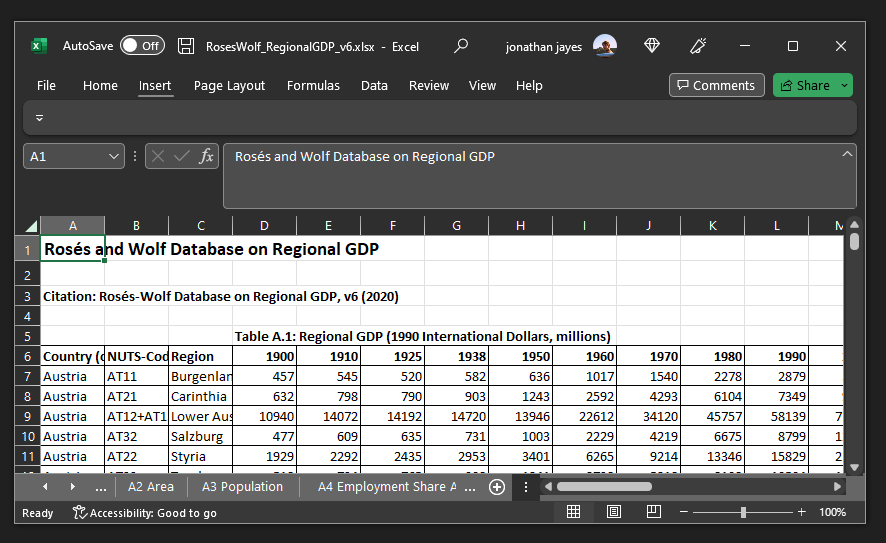
\includegraphics{labs/Lab-1-resources/excel_format.PNG}

}

\caption{Screenshot of excel file}

\end{figure}

What we want to do is import the data from each tab, and append it
together.

\begin{verbatim}
import excel using RosesWolf_RegionalGDP_v6.xlsx, sheet("A1 Regional GDP") firstrow cellrange(A6:O179) clear // import Excel sheet
rename (D E F G H I J K L M N O) (year_1900 year_1910 year_1925 year_1938 year_1950 year_1960 year_1970 year_1980 year_1990 year_2000 year_2010 year_2015)
\end{verbatim}

This is what the data now looks like inside Stata. It is a wide
dataframe, with 173 rows (the number of regions) and 15 variables (3
identifiers and 12 years worth of data)

\begin{figure}

{\centering 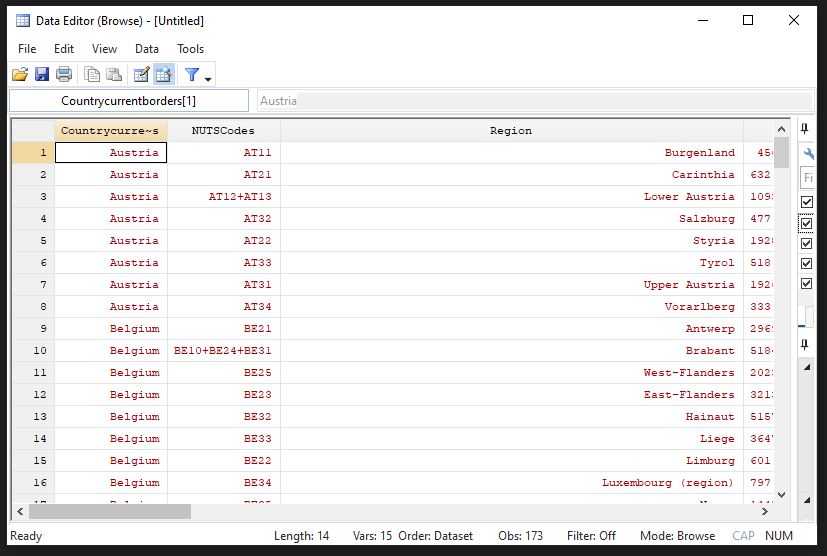
\includegraphics{stata_view_1.PNG}

}

\caption{Screenshot of Stata format}

\end{figure}

\begin{tcolorbox}[enhanced jigsaw, breakable, arc=.35mm, coltitle=black, opacitybacktitle=0.6, colframe=quarto-callout-tip-color-frame, rightrule=.15mm, colbacktitle=quarto-callout-tip-color!10!white, toprule=.15mm, colback=white, toptitle=1mm, bottomtitle=1mm, titlerule=0mm, opacityback=0, left=2mm, leftrule=.75mm, title=\textcolor{quarto-callout-tip-color}{\faLightbulb}\hspace{0.5em}{Tip}, bottomrule=.15mm]

Recall that the Roses Wolf database has geographic data on GDP and
population at the nomenclature of territorial units 2 (NUTS-2) level,
from 1900 to 2015.

\end{tcolorbox}

Next we want to be sure that Stata is reading in the values as numbers
rather than text. For this we use the \texttt{destring} command.

\begin{verbatim}
import excel using RosesWolf_RegionalGDP_v6.xlsx, sheet("A1 Regional GDP") firstrow cellrange(A6:O179) clear allstring `// we import each sheet in the Excel file separately and save it as one file`
rename (D E F G H I J K L M N O) (year_1900 year_1910 year_1925 year_1938 year_1950 year_1960 year_1970 year_1980 year_1990 year_2000 year_2010 year_2015)
destring year_*, replace
\end{verbatim}

If there are non-numerical values in a string you cannot use destring
and should not use the force-option as it would create missing values A
better approach is to check all cases that are non-numerical and replace
them (e.g.~change ``one'' to ``1'')

Other common data cleaning commands could include:

\texttt{//\ tab\ var1\ if\ missing(real(var1))}
\texttt{//\ replace\ var1\ ...\ if\ ...}
\texttt{//\ destring\ var1,\ replace}

Next we want to take the data from a wide format to a long format. A
long format means that each row is an observation, each column is a
variable, and each cell has just one value in it.

\begin{figure}

{\centering 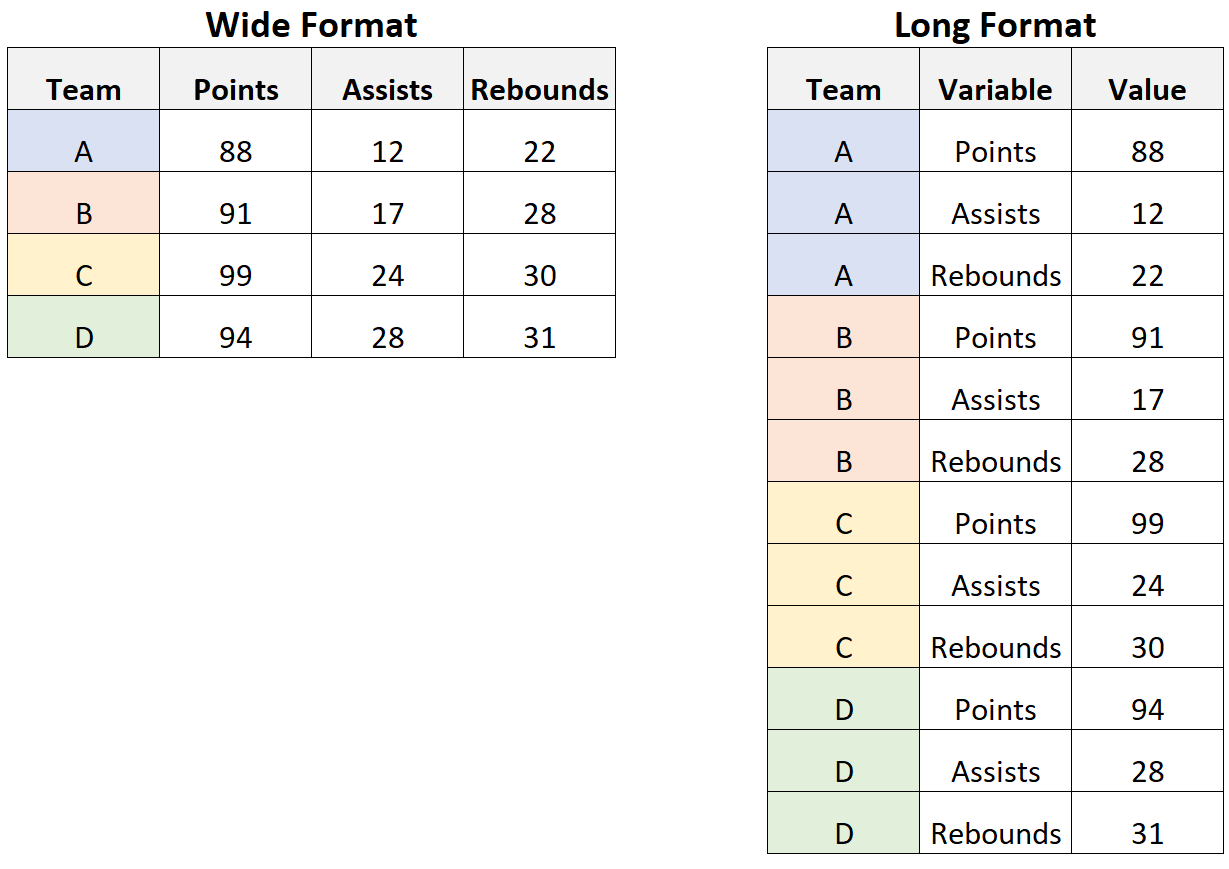
\includegraphics{wide_to_long.png}

}

\caption{Reshape graphic}

\end{figure}

\begin{verbatim}
help reshape
reshape long year_, i(NUTSCodes Region Countrycurrentborder) j(year)
rename year_ regional_gdp_millions
save regional_gdp, replace 
\end{verbatim}

\begin{tcolorbox}[enhanced jigsaw, breakable, arc=.35mm, coltitle=black, opacitybacktitle=0.6, colframe=quarto-callout-tip-color-frame, rightrule=.15mm, colbacktitle=quarto-callout-tip-color!10!white, toprule=.15mm, colback=white, toptitle=1mm, bottomtitle=1mm, titlerule=0mm, opacityback=0, left=2mm, leftrule=.75mm, title=\textcolor{quarto-callout-tip-color}{\faLightbulb}\hspace{0.5em}{Tip}, bottomrule=.15mm]

Never overwrite your raw data - this could be a big problem if you
haven't saved it somewhere else. Good practice is to save a copy of your
data in a different folder before the analysis, and make any changes
through your do-file (e.g.~changing ``one'' to ``1'' in Stata rather
than excel).

\end{tcolorbox}



\end{document}
